\documentclass[11pt, oneside]{article}   	% use "amsart" instead of "article" for AMSLaTeX format
\usepackage{geometry}                		% See geometry.pdf to learn the layout options. There are lots.
\geometry{letterpaper}                   		% ... or a4paper or a5paper or ... 
%\geometry{landscape}                		% Activate for rotated page geometry
%\usepackage[parfill]{parskip}    		% Activate to begin paragraphs with an empty line rather than an indent
\usepackage{graphicx}				% Use pdf, png, jpg, or eps§ with pdflatex; use eps in DVI mode
								% TeX will automatically convert eps --> pdf in pdflatex		
\usepackage{amssymb}

%SetFonts

%SetFonts


\title{CS 161 HW 8}
\author{Ken DENG}
%\date{}							% Activate to display a given date or no date

\begin{document}
\maketitle
%\section{}
%\subsection{}

\section{Question 1:}

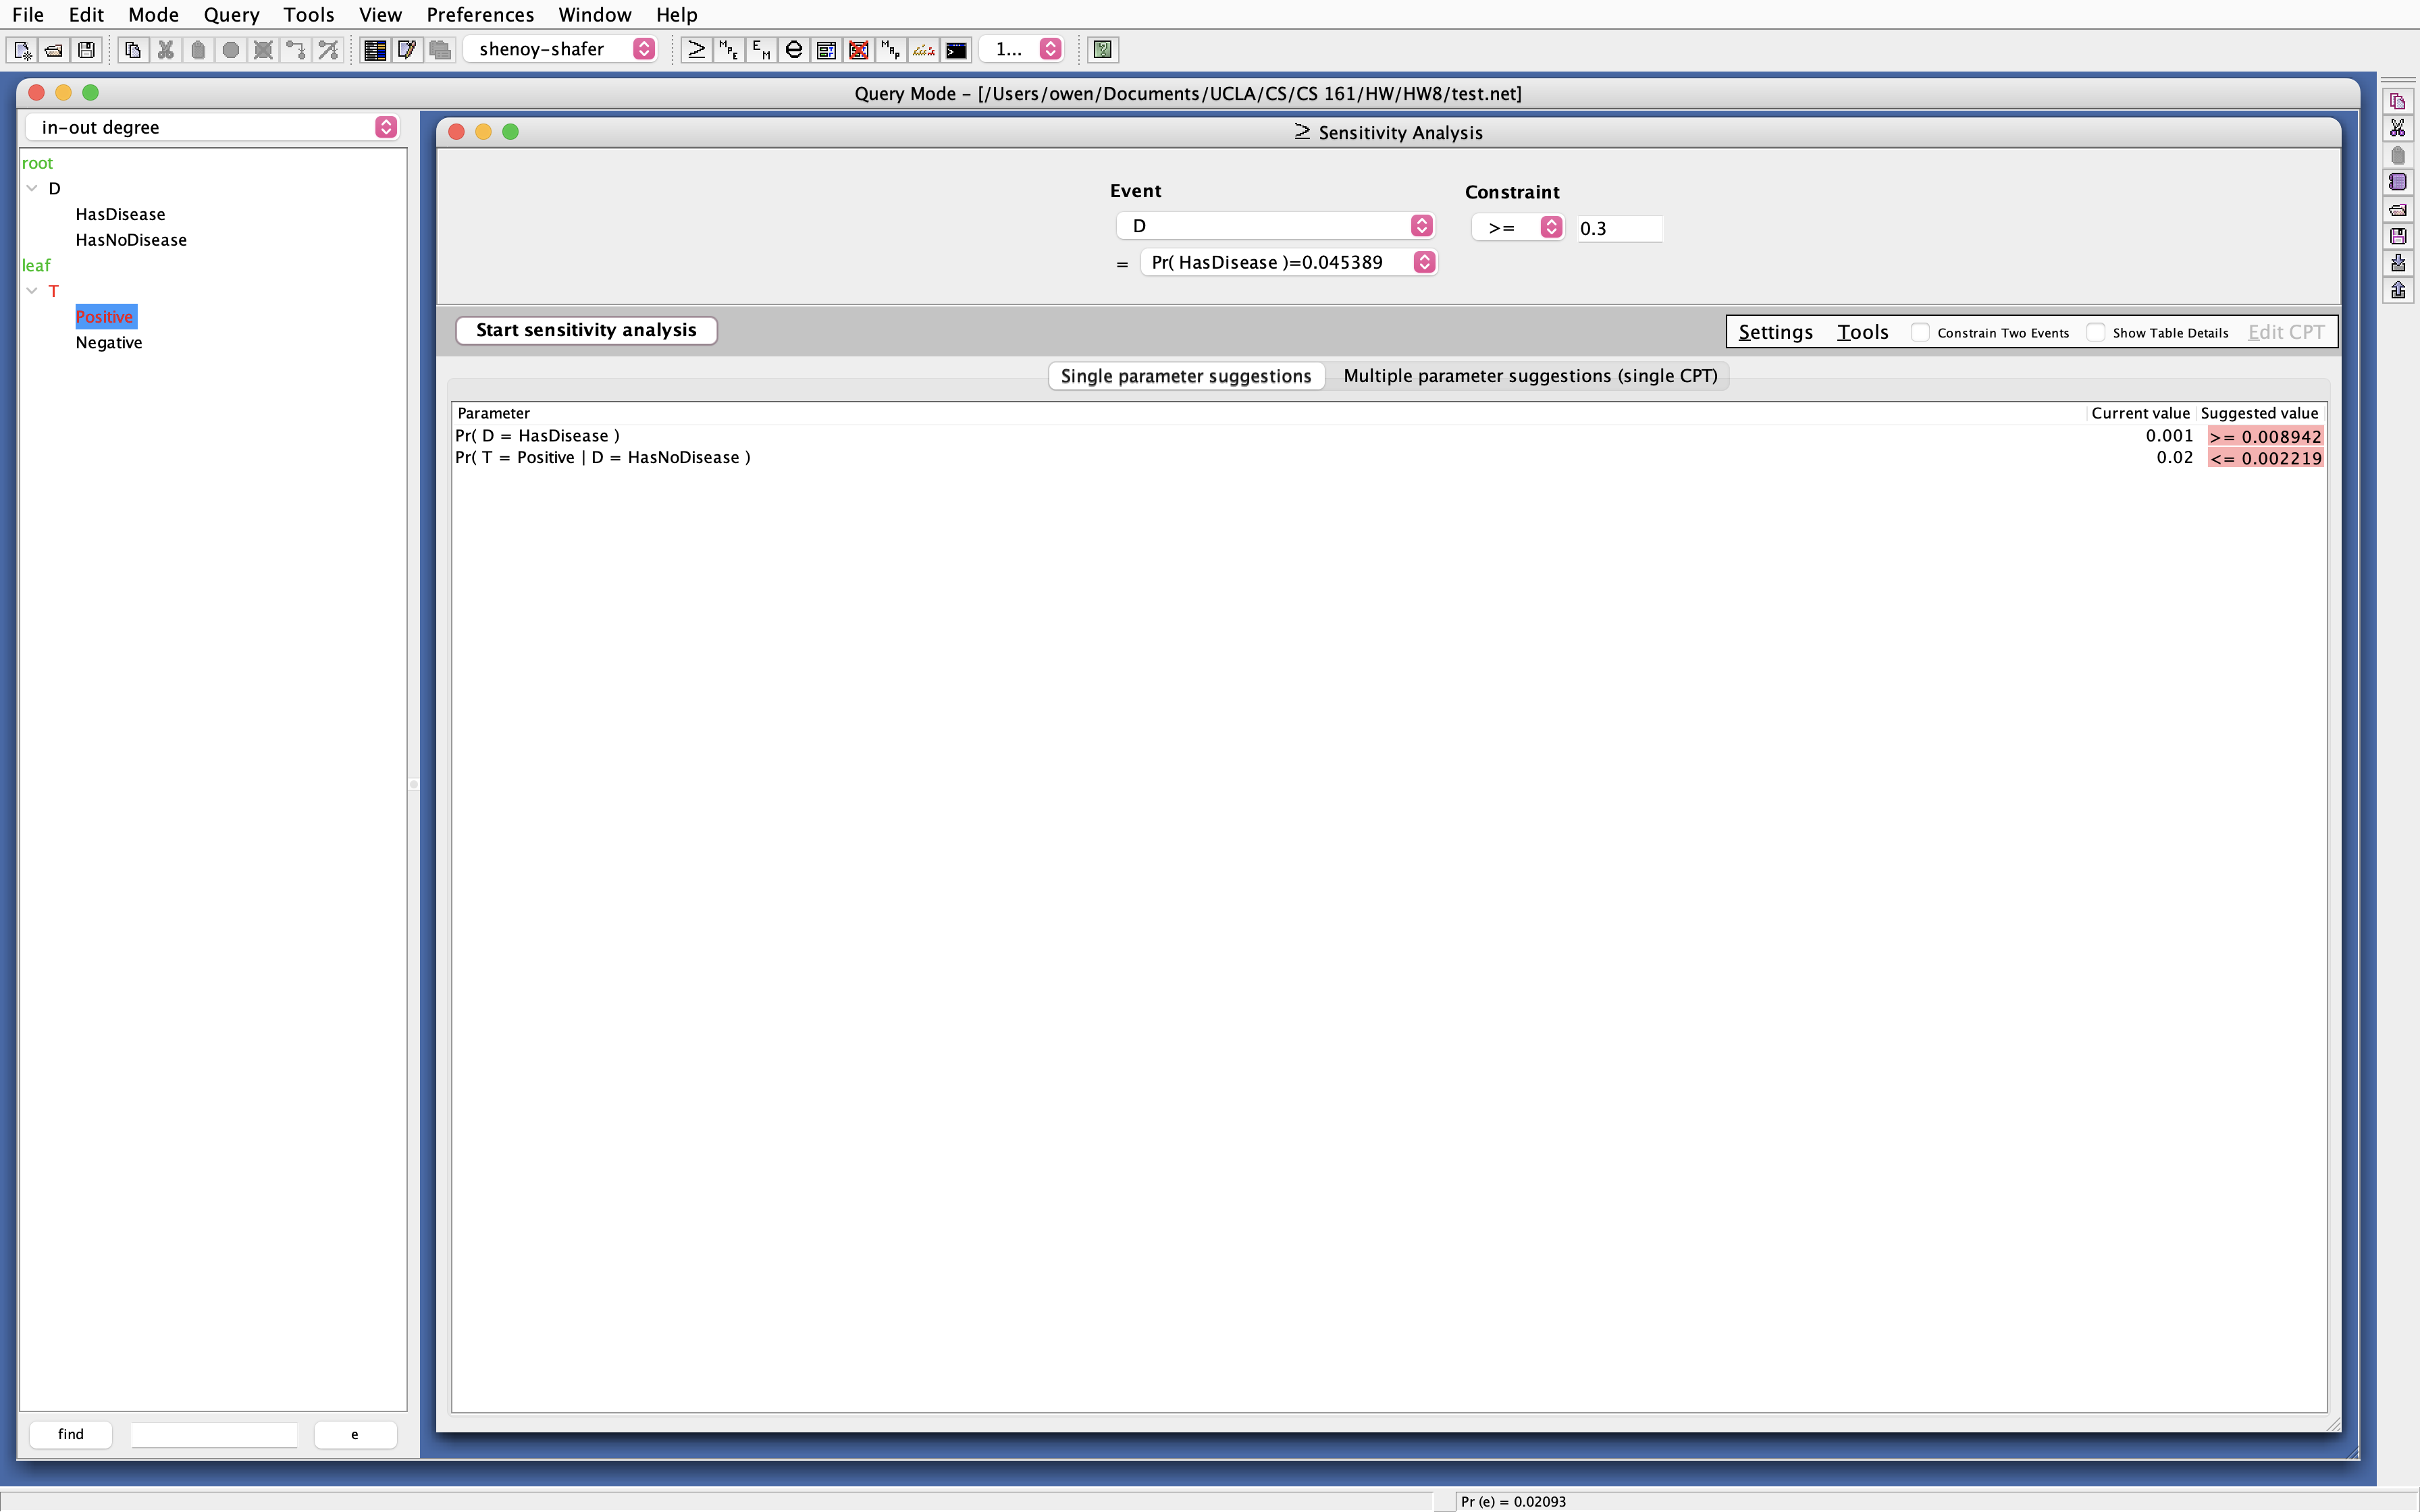
\includegraphics[scale=0.25]{Q1}\\

\noindent{}By the attached image above, we see that in order to ensure that $Pr(D|T) \geq 0.3$:\\
\phantom{aaaa}i. The prior probability of having the disease need to be greater than 0.008942;\\
\phantom{aaaa}ii. The probability of false positive for the test need to be less than 0.002219;\\
\phantom{aaaa}iii. The probability of false negative for the test has no constraint.

\pagebreak 
\section{Question 2:}

\noindent{}\textbf{a.}\\

\noindent{}The set of variables and their values:\\

\noindent ExpectingGuests: Yes/No\\
FamilyHome: Yes/No\\
SoundSensor: On/Off\\
LightSensor: On/Off\\
HearableBarking: Yes/No\\
Battery: OK/Dead\\
SoundSensorHealth: OK/Broken\\
LightSensorHealth: OK/Broken\\
DogBarking: Yes/No\\
DogOutside: Yes/No\\
OutdoorLight: On/Off\\
DogBowelTrouble: Yes/No\\

\noindent{}\textbf{b.}\\

\noindent{}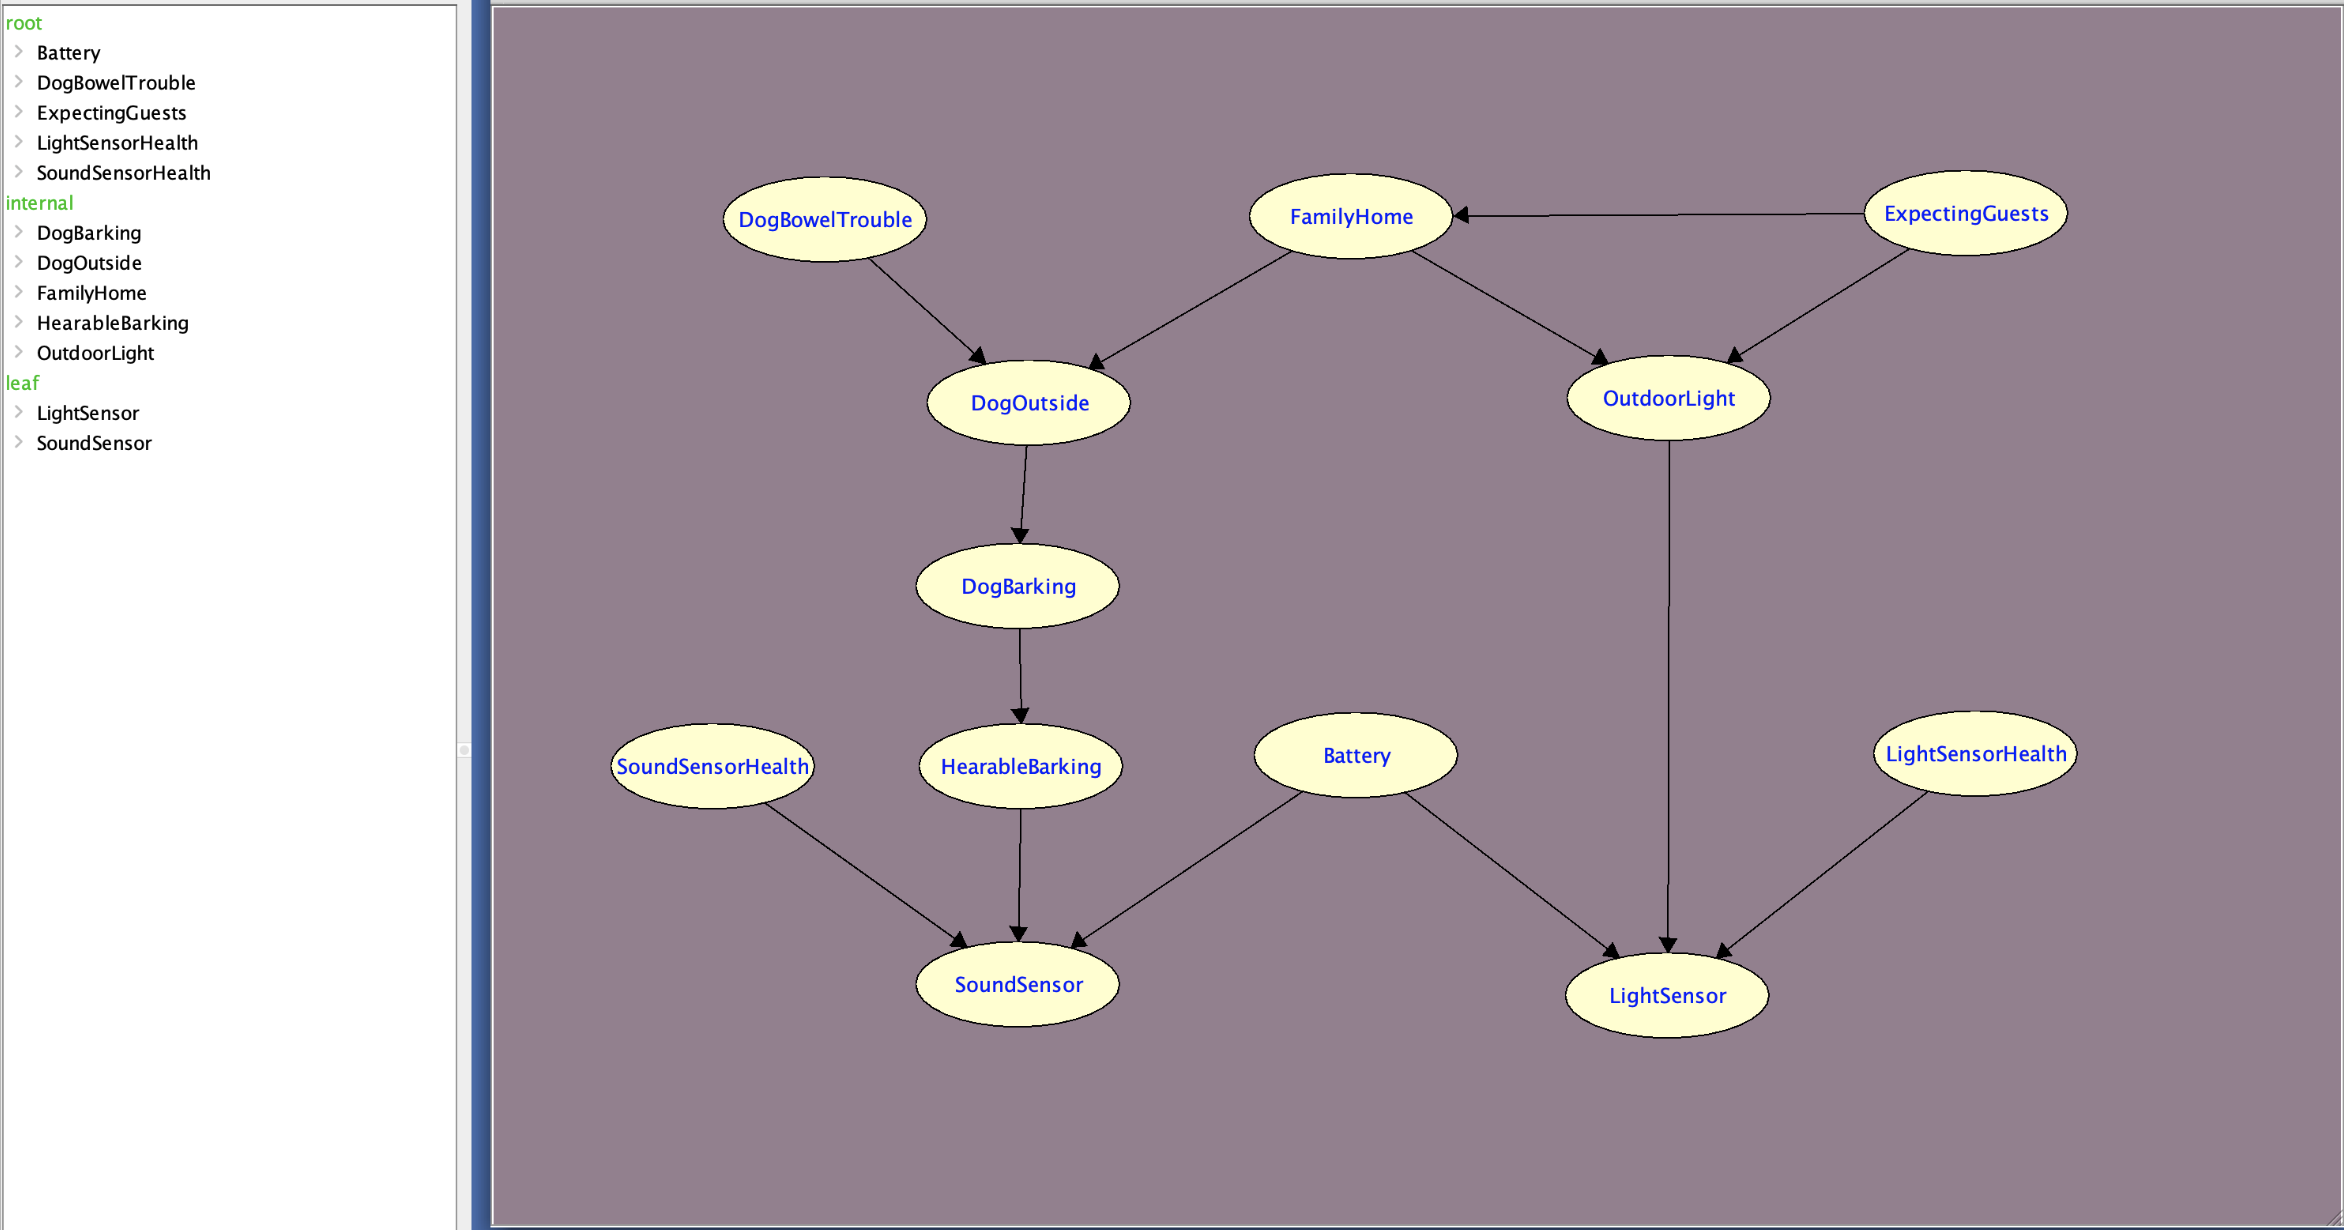
\includegraphics[scale=0.4]{Q2b}\\

\pagebreak
\noindent{}\textbf{c.}\\

\noindent{}i. \\

\noindent{}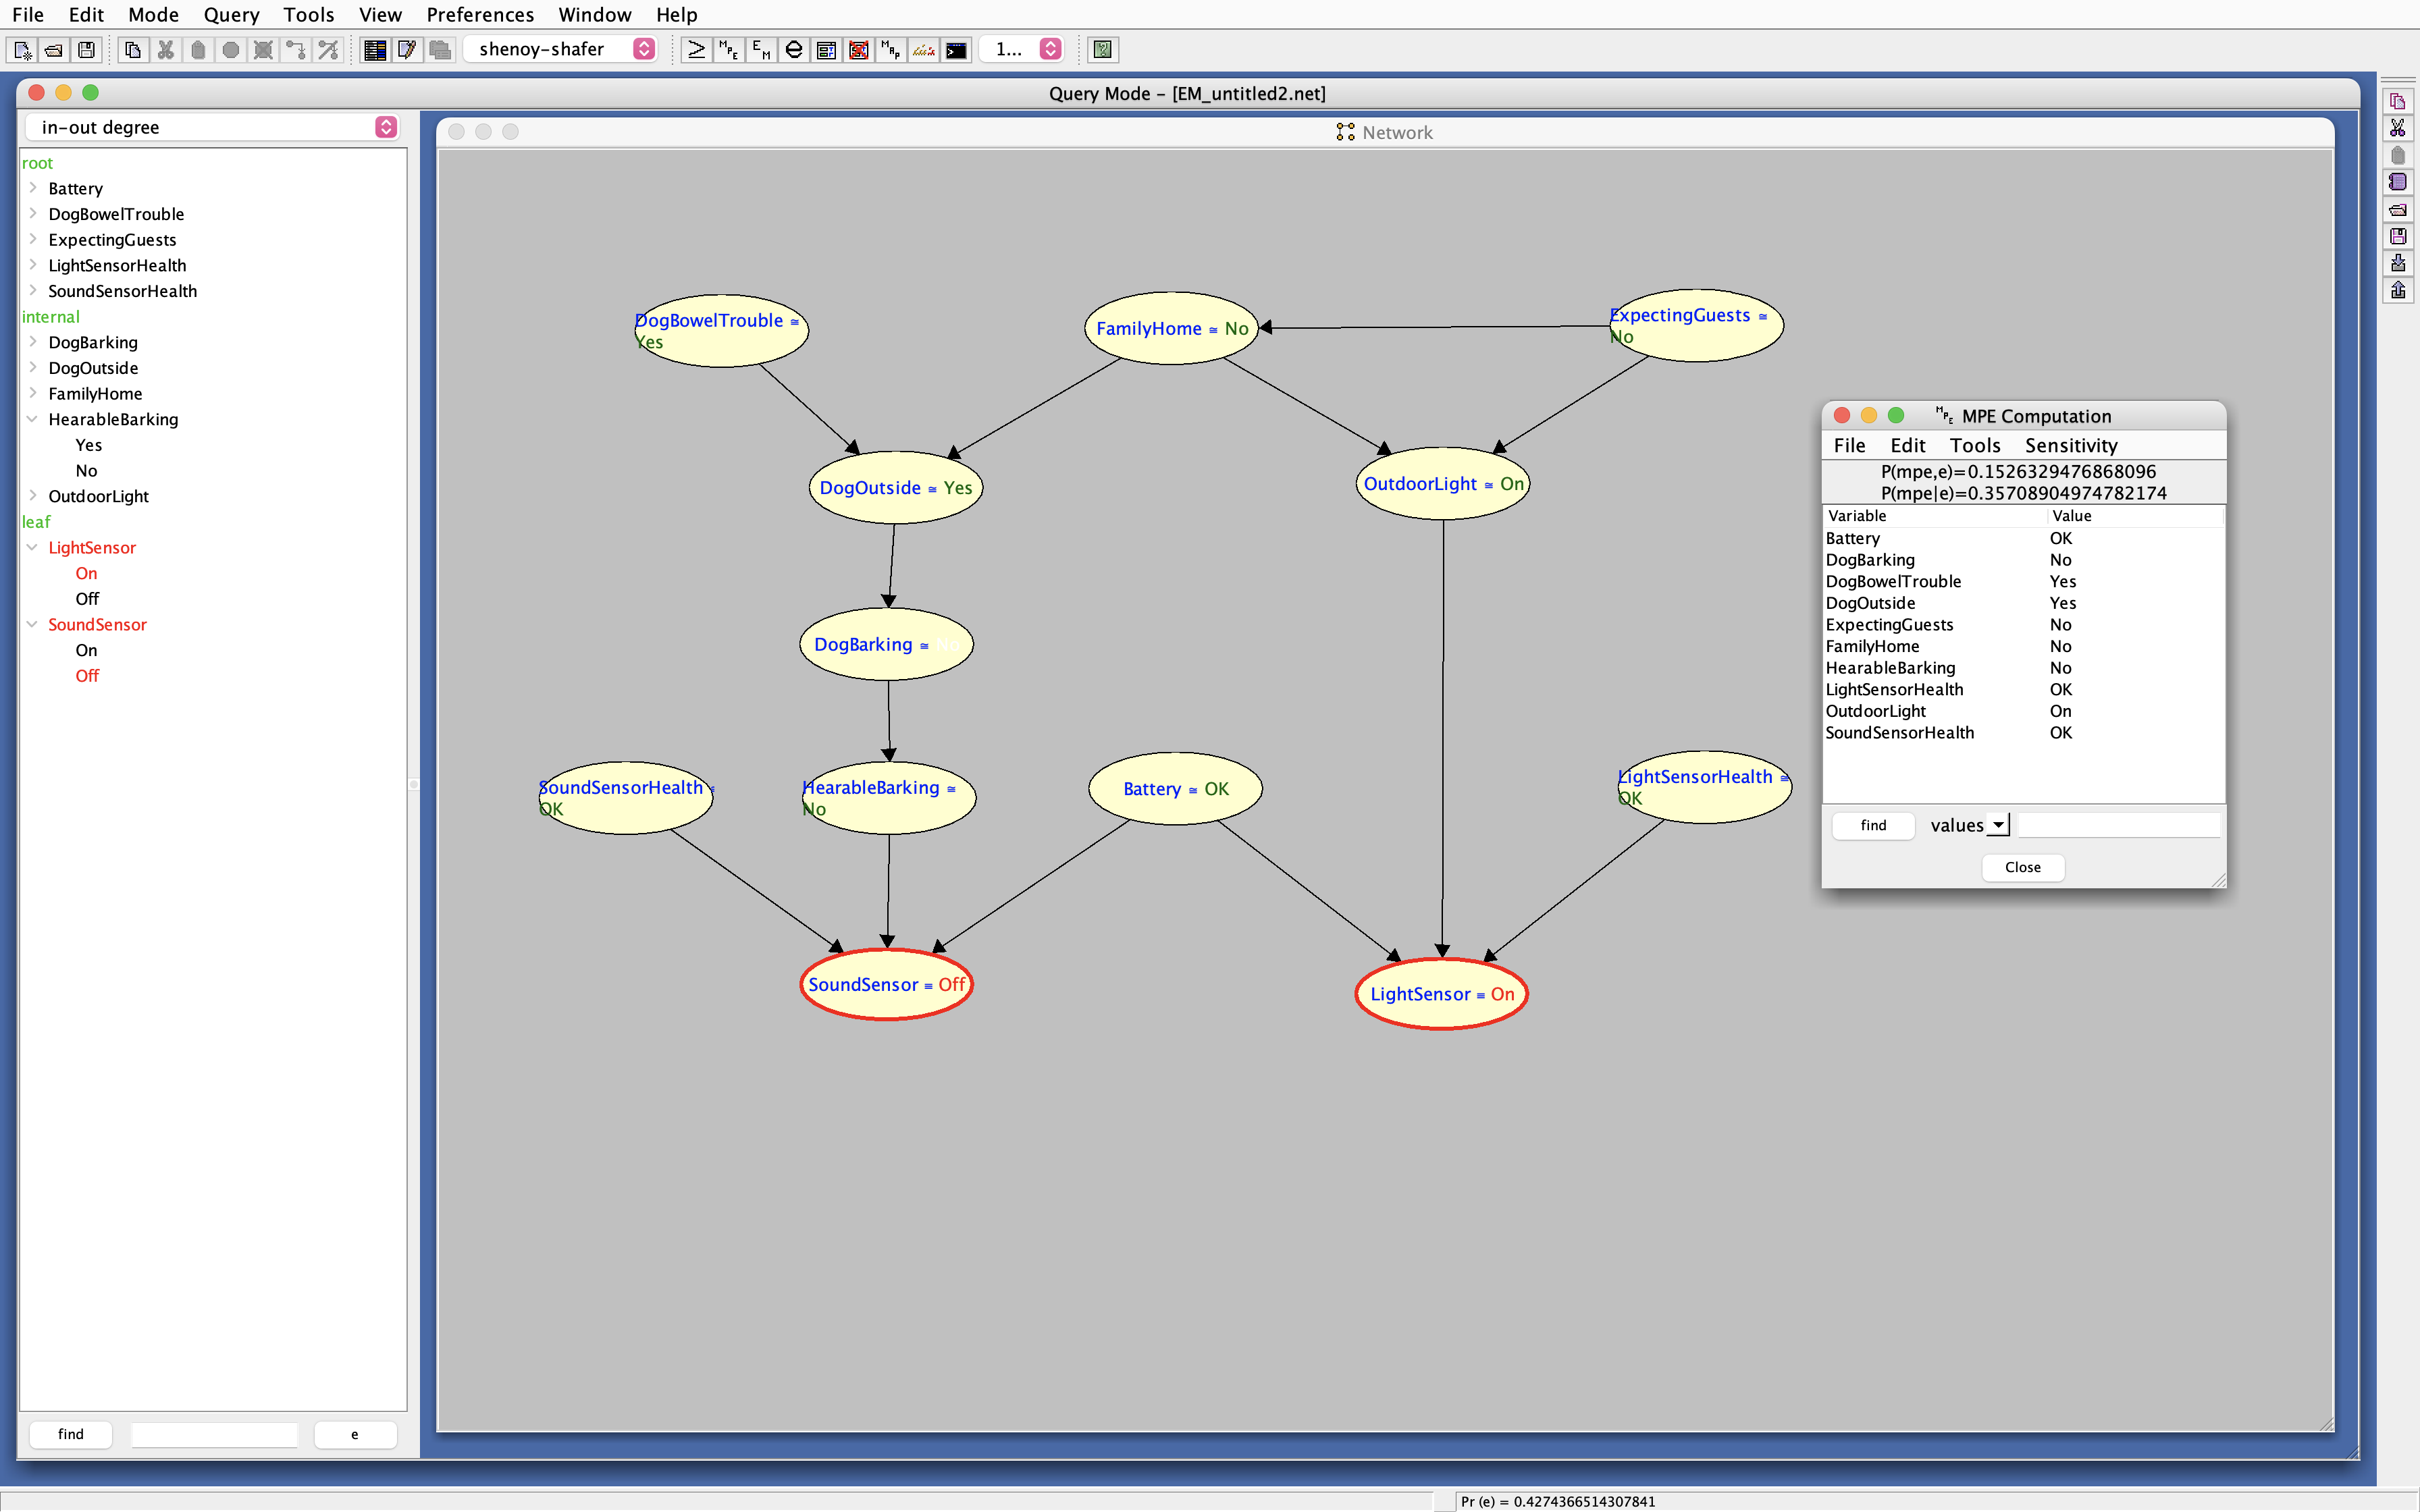
\includegraphics[scale=0.25]{Q2ci}\\

\noindent After running the EM algorithm, I switched into Query Mode and set the variable ``SoundSensor = Off" and ``LightSensor = On". Then in the Query Menu Tab I used MFE Computation to get the result shown in the diagram above, which indicates that the most likely instantiation of all other variables are ``Battery = OK", ``DogBarking = No", ``DogBowelTrouble = Yes", ``DogOutside = Yes", ``EspectingGuests = No", ``FamilyHome = No", ``HearableBarking = No", ``LightSensorHealth = Ok", ``OutdoorLight = On", and ``SoundSensorHealth = OK".\\

\pagebreak 
\noindent{}ii. \\

\noindent{}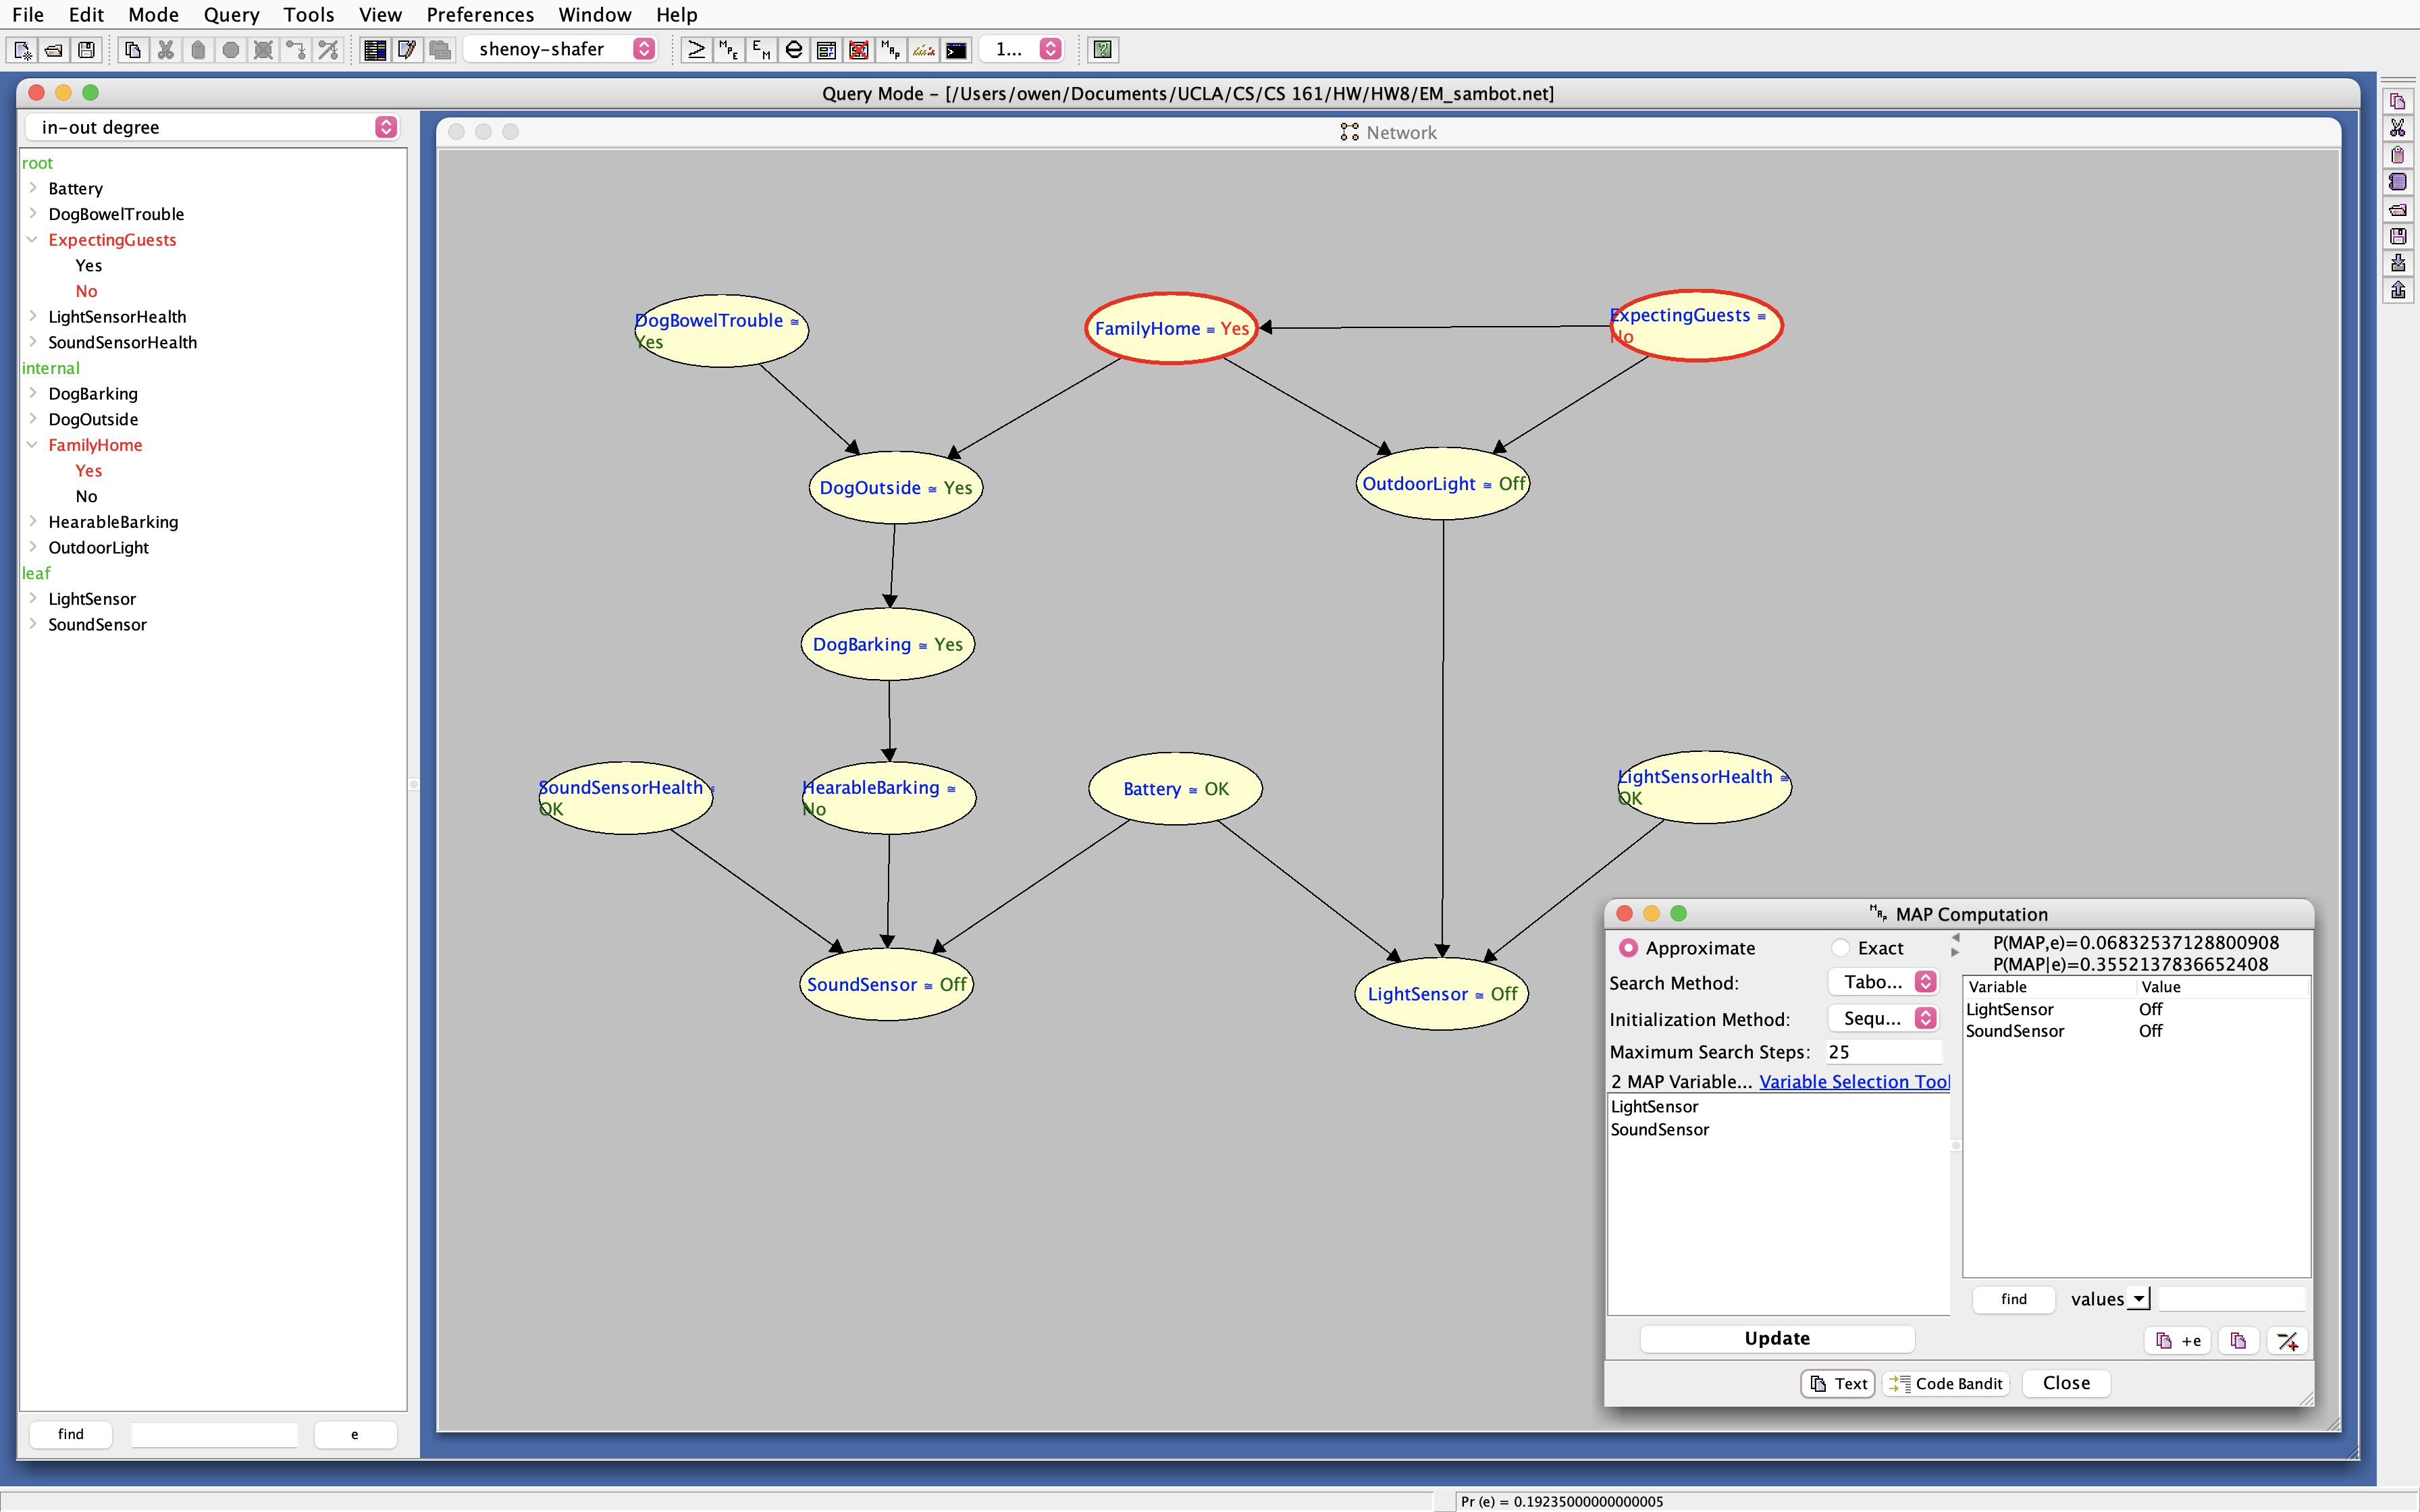
\includegraphics[scale=0.25]{Q2cii}\\

\noindent After running the EM algorithm, I switched into Query Mode and set the variable ``FamilyHome = Yes" and ``ExpectingGuest = No". Then I used MAP Computation and used Variable Selection Tool to select the variables ``LightSensor" and ``SoundSensor". Finally, I derived the results as shown in the image above, which indicates that the most likely instantiation for sensors are ``LightSensor = Off" and ``SoundSensor = Off".\\

\pagebreak 
\noindent{}iii. \\

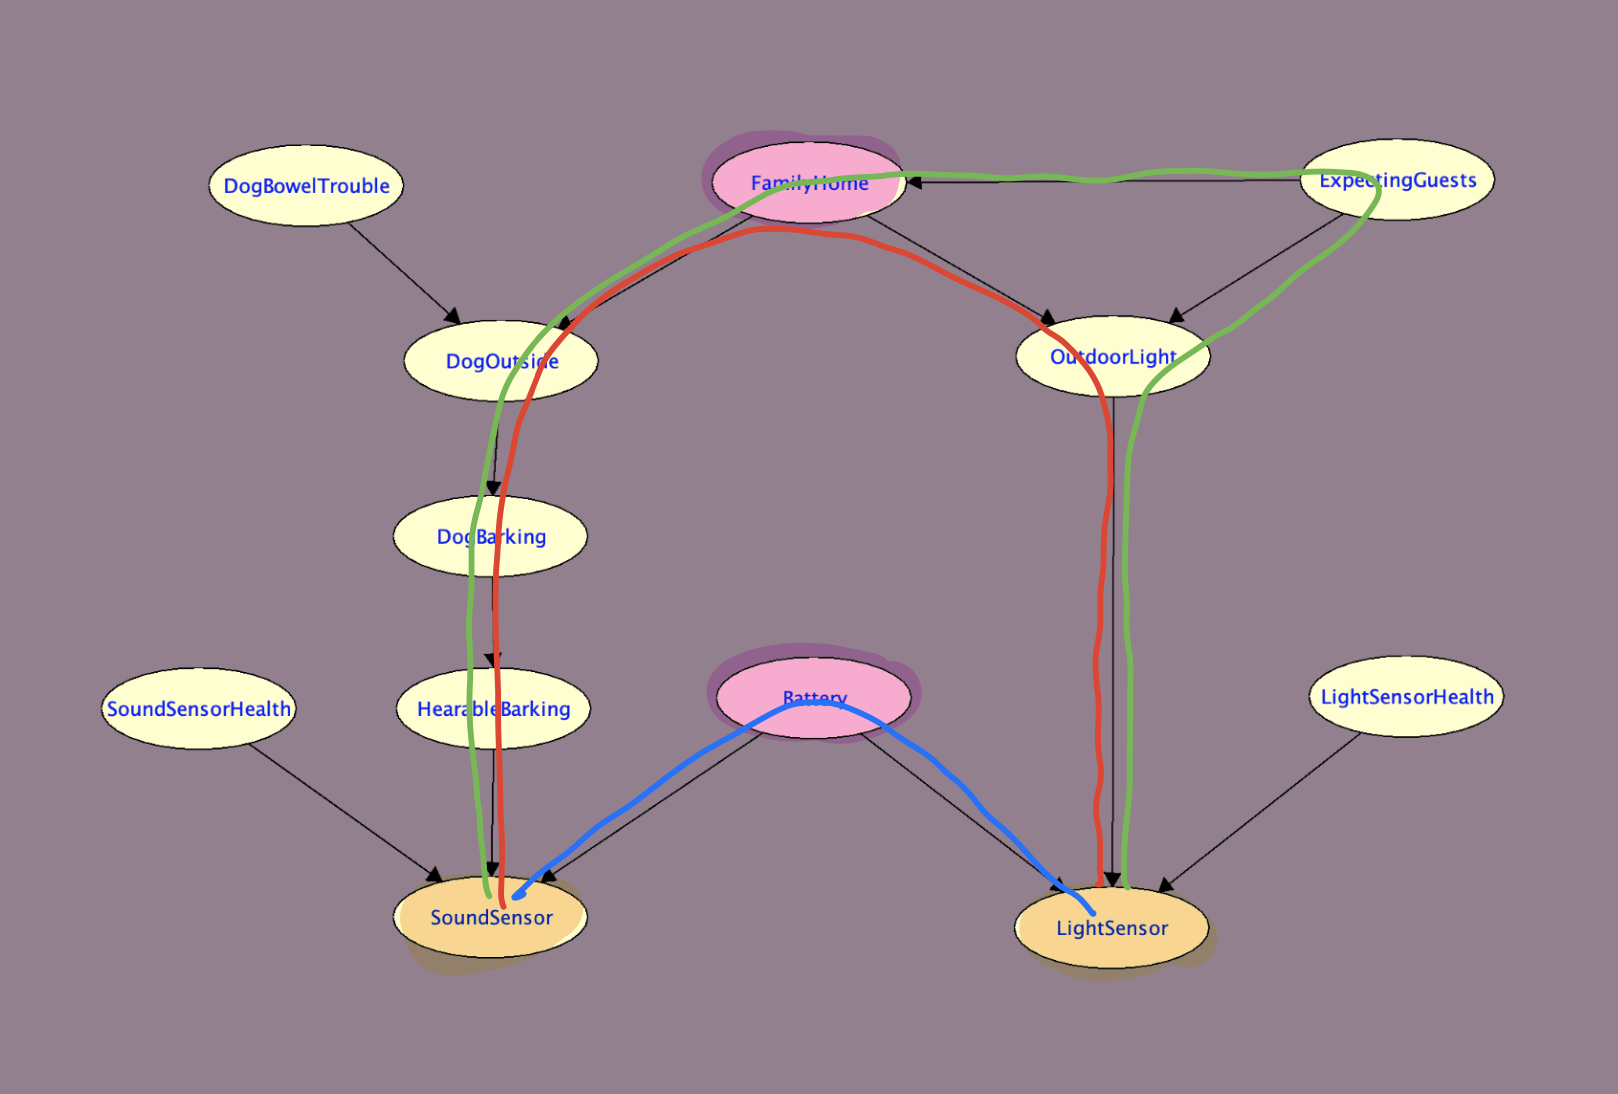
\includegraphics[scale=0.5]{Q2ciii}\\

\noindent The smallest set is $Z = \{FamilyHome, Battery\}$.\\

\noindent Consider the three possible paths:\\

\noindent\phantom{aaaa}For the blue path, we see that $\textrm{SoundSensor} \leftarrow \textrm{Battery} \rightarrow \textrm{LightSensor}$ is a divergent\\\phantom{aaaa}valve, and since $\textrm{Battery} \in Z$, we see this valve is closed, and hence this path is blocked.\\

\noindent\phantom{aaaa}For the green path, we see that $\textrm{ExpectingGuests} \rightarrow \textrm{FamilyHome} \rightarrow \textrm{DogOutside}$ is a \\\phantom{aaaa}sequential valve, and since $\textrm{FamilyHome} \in Z$, we see this valve is closed, and hence \\\phantom{aaaa}this path is blocked.\\

\noindent\phantom{aaaa}For the red path, we see that $\textrm{DogOutside} \leftarrow \textrm{FamilyHome} \rightarrow \textrm{OutdoorLight}$ is a \\\phantom{aaaa}divergent valve, and since $\textrm{Familyhome} \in Z$, we see this valve is closed, and hence this \\\phantom{aaaa}path is blocked.\\

\noindent Since all three possible paths are blocked, we see that the two sensors are independent given $Z = \{FamilyHome, Battery\}$.

\pagebreak 
\noindent{}iv. \\

\noindent{}The type of network you constructed is a multiply-connected network, as there are multiple paths between two nodes.\\

\noindent{}For instance, between the nodes ``ExpectingGuests" and ``OutdoorLight", there are two paths:\\
\noindent{}\phantom{aaaa}$\textrm{ExpectingGuests} \rightarrow \textrm{FamilyHome} \rightarrow \textrm{OutdoorLight}$\\
\noindent{}\phantom{aaaa}$\textrm{ExpectingGuests} \rightarrow \textrm{OutdoorLight}$\\




\end{document}  



















